\documentclass[10pt]{article}
\usepackage[margin=0.85in]{geometry}
\usepackage[T1]{fontenc}
\usepackage{amsmath,amssymb,amsthm,booktabs,graphicx,float,hyperref}
\usepackage{microtype}
\usepackage[section]{placeins}
\renewcommand{\topfraction}{0.9}
\renewcommand{\textfraction}{0.08}
\renewcommand{\floatpagefraction}{0.8}
\newtheorem{proposition}{Proposition}
\newtheorem{conjecture}{Conjecture}
\newcommand{\ForwardMAE}{0.00924}
\newcommand{\ReverseMAE}{0.03694}
\newcommand{\RoundtripMAE}{1.46\times10^{-7}}
\newcommand{\WorstError}{2.92\times10^{-6}}
\newcommand{\ExactRate}{100.0}
\newcommand{\MinMinutes}{2.4}
\newcommand{\MaxMinutes}{2.5}
\newcommand{\MinVRAM}{380}
\newcommand{\MaxVRAM}{380}
\newcommand{\OldTargetMAE}{0.04924}
\newcommand{\NewTargetMAE}{0.04618}
\newcommand{\OldCorrelation}{0.1195}
\newcommand{\NewCorrelation}{0.0515}

\title{Learning Reversible Stochastic Tensor Transformations:\\A Path Toward Quantum-Proof MultiModal Encryption}
\author{Samuel Cavazos\\Chief Data Scientist, \href{https://alshival.ai}{Alshival.Ai}}
\date{October 2026}
\begin{document}
\maketitle
\begin{abstract}
Protecting personal communication and sensitive medical and scientific data is
a central motivation for encryption research. A tensor-algebraic perspective
offers a common mathematical language for studying transformations of images,
audio, and other structured data. The source and transmitted carrier
need not share a modality: text could be carried as an image, or an image as
audio, while a corresponding inverse recovers the original data. We explore
this possibility as a foundation for future multimodal privacy systems,
beginning with reliable recovery in an image-to-image experiment.
Our initial study learned forward and reconstruction maps independently,
without guaranteed inversion or held-out evaluation. Here we introduce a structural constraint:
reversible coupling blocks provide an explicit inverse, while training learns
to approximate a prescribed stochastic endpoint. A compact, 44,296-parameter
network targets a 32-step Gaussian process, transforms all RGBA channels, and
uses unclipped floating-point payloads to avoid destructive byte conversion.
Three runs of 2,000 optimizer updates use 647 training, 81 validation, and 81 test
Pok\'emon sprites; the test set was previously examined during exploratory work.
Mean test forward- and reverse-target MAEs are
\ForwardMAE{} and \ReverseMAE{}, respectively; mean learned round-trip error is
$\RoundtripMAE$. Exact whole-image RGBA recovery reaches \ExactRate\% after
rounding in every tested run and domain. Target approximation is learned, whereas
round-trip recovery relies on constructed inversion and numerical precision.
A separate proof sketch shows how a reversible learned carrier can preserve
one-time-pad secrecy against classical and quantum observation. This provides
a conditional route toward the future-system conjecture; confidentiality of
the experimental Gaussian transform remains unestablished.
\end{abstract}

\section{Theory: tensor maps, stochastic endpoints, and recovery}
The motivating question is whether we can learn to transform data into another
representation while retaining a reliable way to recover its original values.
That representation could have a different apparent modality: a message could
travel as an image, or an image as an audio signal. This separates what the data
originally means from the form that carries it.

The overarching idea begins with an invertible map $F:\mathcal X\to\mathcal Y$
between tensor representations. We train a model $\sigma$ to approximate the
forward map and a model $\tau$ to approximate its inverse:
\begin{equation*}
 \sigma(x)\approx F(x),\qquad
 \tau(y)\approx F^{-1}(y),\qquad
 \tau(\sigma(x))\approx x.
\end{equation*}
The first two relations express agreement with the desired transformations;
the third asks whether the learned models work together to recover the input.
Two independently learned approximations need not be exact inverses of one
another. Our initial Encrypter--Decrypter study \cite{original} learned the
directions independently. Here we constrain the models to share an explicit
inverse. We write $\sigma_\theta$ and $\tau_\theta$ when showing their shared
parameters $\theta$ explicitly. Training adjusts both directions, while the
architecture guarantees $\tau_\theta=\sigma_\theta^{-1}$ in exact arithmetic.

For our image-to-image experiment, we choose $F$ from a stochastic process
that progressively attenuates an image and adds Gaussian noise. Once the
realized noise field $n$ is fixed, the 32-step endpoint is an invertible map
$F_n(x)=0.25x+n$, with inverse $F_n^{-1}(y)=(y-n)/0.25$. Supplying the same
$n$ in both directions gives a controlled target whose forward and inverse
operations are known, so we can measure target approximation separately from
recovery of the network's own output. We show the conditioning input explicitly
as $\sigma_\theta(x,n)$ and $\tau_\theta(y,n)$; the inverse relation holds for
each fixed $n$.

Figure~\ref{fig:mew-learned-map} shows these two learned directions using Mew:
$\sigma$ transforms the sprite and $\tau$ recovers its original pixel values.
\begin{figure}[!htbp]
\centering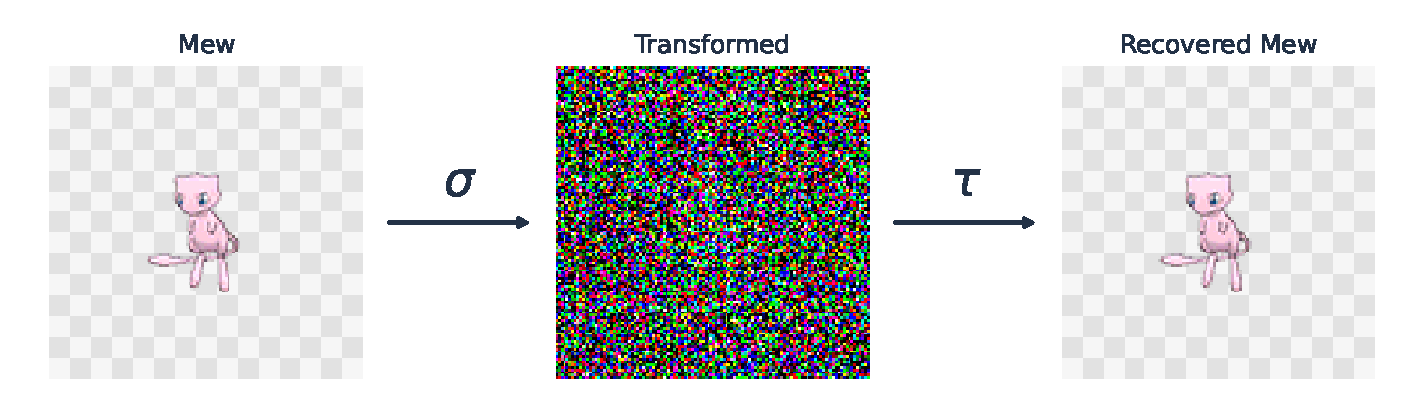
\includegraphics[width=\linewidth]{generated/mew-learned-map.pdf}
\caption{Mew through the learned forward map $\sigma$ and its constructed inverse
$\tau$, using the frozen seed-17 model trained for 2,000 updates on the 32-step
target. Both directions receive the same saved noise field. The middle panel
shows a clipped RGB preview; recovery uses the full floating-point RGBA payload.
Every original RGBA byte is recovered after rounding. Mew is a training image
chosen to illustrate the maps; Section~3 reports the held-out results.}
\label{fig:mew-learned-map}
\end{figure}

This learning objective can be posed for other invertible maps, including
maps between modalities; the stochastic process is our chosen test case.
Its extension to a particular map requires suitable tensor encodings, model
capacity, training data, and storage precision. Different target maps may also
require different reversible architectures.
The theory below develops this tensor-map viewpoint through composition,
smooth changes of coordinates, and a polynomial specialization. Section~2
relates recovery to the longer-term encryption objective, and Section~3 reports
the experiments. Multimodal operation and cryptographic security remain research
goals; the experiments concern image transformations and numerical recovery.

\subsection{A modality-independent formulation}
A digital image is a table of numbers. Our Mew sprite has four values at each
of $120\times120$ positions: red, green, blue, and transparency. Arranging these
values into a tensor gives us a precise way to describe how a transformation
changes them. Audio can likewise be indexed by time and channel, and video by
frame, channel, and spatial position. Tensor representations let us reason about
maps between these forms as well as maps within one form. Each modality still
needs its own suitable encoding and model.

Let $\mathcal X\subseteq\mathbb R^{d_1\times\cdots\times d_k}$ be a set of data
tensors. For digital data, $\mathcal X$ may be a finite lattice; it need not itself
be a vector space. An image is one instance, with spatial axes and color channels.
Waveforms, spectrograms, video, and token sequences admit other tensor encodings.
This common representation permits a shared mathematical formulation, while
architecture, shape handling, and output constraints remain modality dependent.
Exact recovery of the source data additionally requires the initial tensor
encoding to be lossless: a lossy embedding cannot be inverted merely because a
later tensor transform is invertible.

The original paper's tensor-map language \cite{original} becomes more precise
when we distinguish the stored data from its ambient space. For our images,
\begin{equation*}
 V=\mathbb R^4\otimes\mathbb R^H\otimes\mathbb R^W
 \cong\mathbb R^N,\qquad N=4HW=57{,}600.
\end{equation*}
The tensor-product notation $\otimes$ records the channel, height, and width
axes.
An entire sprite is one point in this space, with a coordinate for each channel
value at each pixel. Byte-valued sprites occupy a finite grid inside $V$;
differential geometry describes the smooth maps we extend to the surrounding
real coordinates. Here the tensor-algebraic viewpoint concerns these tensor
spaces and the composition of maps between them. Our learned maps can be
nonlinear and need not preserve vector addition or tensor products.

\paragraph{The source and carrier can have different forms.}
Consider the text \texttt{MEW}. A proposed encoder could represent its exact
text bytes through the pixel values of an image; the corresponding decoder
would recover \texttt{MEW} from those values. The image need not display the
letters or depict the message's meaning. Similarly, an encoder could carry
Mew's RGBA pixel values in audio samples, with a decoder reconstructing the
original sprite from the waveform. The sound need not describe Mew. The aim
is to preserve the source information while changing its outward form, as
illustrated in Figure~\ref{fig:cross-modal}.

\begin{figure}[!htbp]
\centering
\renewcommand{\arraystretch}{1.8}
\begin{tabular}{ccccc}
\shortstack{Text source\\\texttt{MEW}} & $\xrightarrow{\text{encode}}$ &
\shortstack{Image carrier\\pixel values} & $\xrightarrow{\text{decode}}$ &
\shortstack{Recovered text\\\texttt{MEW}} \\
\shortstack{Image source\\Mew's RGBA pixels} & $\xrightarrow{\text{encode}}$ &
\shortstack{Audio carrier\\waveform samples} & $\xrightarrow{\text{decode}}$ &
\shortstack{Recovered image\\the same RGBA pixels}
\end{tabular}
\caption{Proposed transformations between modalities. The middle object carries
the source information in a different form; the decoder recovers the original
data, rather than generating a related description or approximation. Any noise,
format metadata, and future secret-key inputs required by the design must also
be available to the decoder.}
\label{fig:cross-modal}
\end{figure}

For source modality $A$ and carrier modality $B$, this extends the recovery
objective to
\begin{equation}
 \tau_{B\to A}(\sigma_{A\to B}(x,n),n)=x,\qquad x\in\mathcal X_A,
 \label{eq:cross-modal}
\end{equation}
where $n$ denotes any conditioning noise shared by the two directions. For
fixed $n$, distinct source inputs must remain distinguishable in the stored
carrier. Its capacity and precision must therefore accommodate the admitted
source data and the agreed format metadata. Lossless source encoding, compatible
tensor shapes, and storage that retains the encoded distinctions are necessary;
a modality change cannot restore information lost through lossy compression.
Equation~\ref{eq:cross-modal} is a design objective for these extensions.

Changing the carrier format alone does not require machine learning. The
learning opportunity is to shape the carrier's visual or acoustic properties
while retaining recoverability. For example, the target might be an ordinary-looking
image rather than an arbitrary array of pixels. Related neural data-hiding work,
such as HiDDeN, learns to embed messages in cover images and recover them with
a decoder \cite{hidden}. Whether a carrier resembles ordinary media, hides the
source modality, or protects the content from an adversary requires separate
evaluation. We begin with image-to-image recovery as a test of the underlying
forward and inverse maps.

\FloatBarrier
To connect this formulation to training, consider the two paths in
Figure~\ref{fig:process-overview}. A prescribed formula generates the training
target; we call this formula the \emph{teacher}. A neural network learns to
approximate that target. Its decoder is constructed to undo the network's own
output, and we also test how it handles the teacher's output. The same realized
noise field is supplied wherever $n$ appears, including during decoding.
The receiver reads this field from the saved record.
\begin{figure}[!htbp]
\centering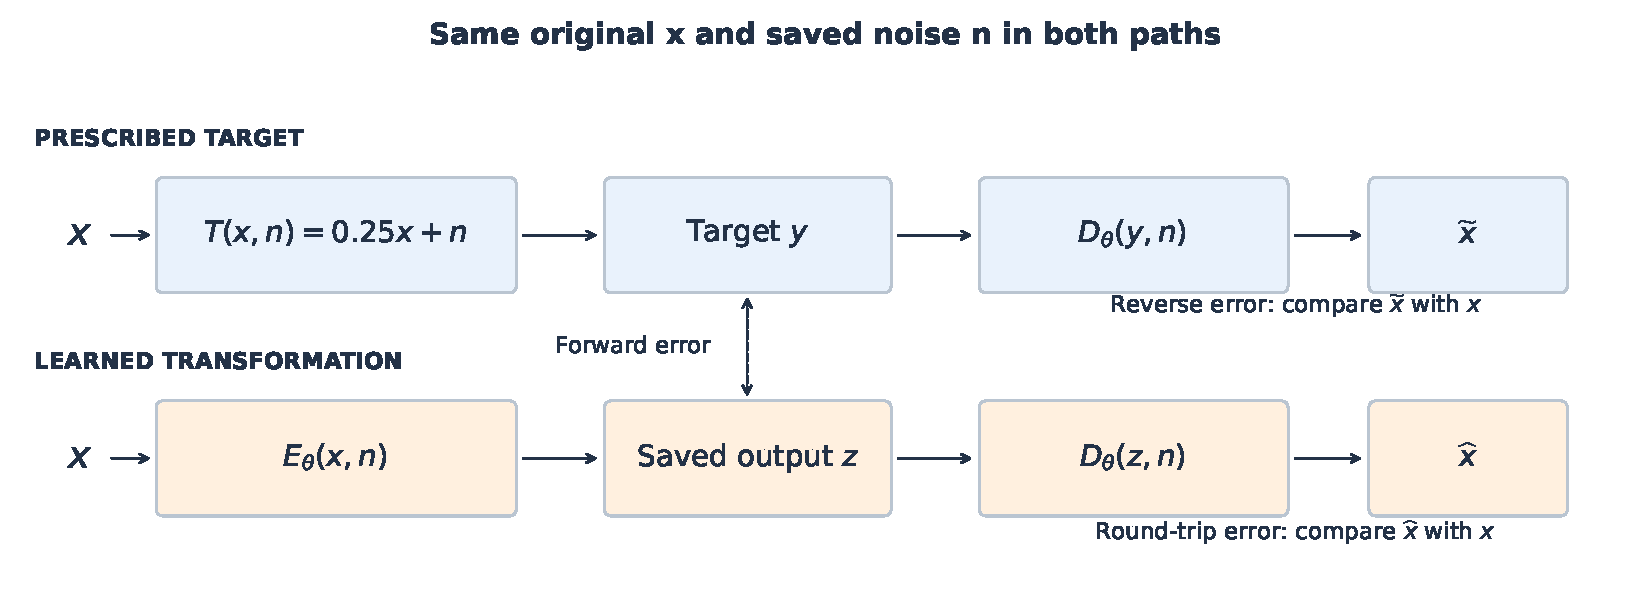
\includegraphics[width=\linewidth]{generated/process-overview.pdf}
\caption{Two paths through the experiment. The upper path creates the prescribed
target and tests its reconstruction; the lower path creates, stores, and reverses
the learned output. Forward error compares the paths' outputs, reverse error
tests the decoder on the teacher's output, and round-trip error tests recovery
from the network's own output. The teacher's 32 stochastic steps are represented
by their endpoint formula; the learned encoder contains four coupling blocks.}
\label{fig:process-overview}
\end{figure}

Write a stochastic family as $T_\omega:\mathcal X\to\mathcal Y$, where $\omega$
specifies a noise realization. For fixed $\omega$, it is an ordinary deterministic
map. Our learned encoder and decoder satisfy the design objectives
\begin{equation}
 \sigma_\theta(x,n)\approx T_\omega(x),\qquad
 \tau_\theta(\sigma_\theta(x,n),n)\approx x,
 \label{eq:objectives}
\end{equation}
where $n$ summarizes the realized noise. In our experiment, $T_\omega=F_n$:
the stochastic teacher is the fixed-noise map introduced at the start of this
section. The decoder is the encoder's constructed
inverse, with shared parameters. Section~\ref{sec:geometry} develops the
geometric and algebraic meaning of this inverse.
Because Gaussian outputs are unbounded, $\mathcal Y$ contains real-valued tensors
and is larger than the bounded image domain.

\FloatBarrier
\subsection{The 32-step stochastic process}
The original process corrupted RGB while preserving alpha, leaving the sprite's
silhouette directly available \cite{original}. We now transform all four RGBA
channels so that recovery includes transparency and no unchanged alpha mask is
carried through the payload. This removes that particular source of leakage;
it does not establish confidentiality.
Each step slightly shrinks the current values and adds a fresh field of random
perturbations. For normalized input $x_0=x\in[0,1]^{4\times H\times W}$, this is
\begin{equation}
 x_t=\sqrt{1-\beta}\,x_{t-1}+\sqrt\beta\,\varepsilon_t,
 \qquad \varepsilon_t\overset{\mathrm{iid}}\sim\mathcal N(0,I).
\end{equation}
Here iid means independent and identically distributed: each step draws a fresh
noise field from the same distribution. The notation $\mathcal N(0,I)$ specifies
Gaussian noise with mean zero and identity covariance, so its entries are
independent and each has unit variance. The parameter $\beta$ controls how much
the current values shrink and how strongly the new noise enters.

The original paper used 1,000 steps with a varying noise schedule, leaving a
signal coefficient of approximately $5.07\times10^{-12}$ before clipping and
byte quantization \cite{original}. Such extreme attenuation made numerical
recovery fragile even before those lossy storage operations. Our subsequent
exploratory study used a constant schedule with a 16-step signal coefficient of
$0.5$. The present experiment retains that exploratory per-step strength
$\beta=1-0.5^{2/16}\approx0.082996$ and increases $T$ from 16 to 32.
Set $a_T=(1-\beta)^{T/2}$. Then $a_{16}=0.5$ and $a_{32}=0.25$.
The integer $T$ counts stochastic-process steps, independently of training updates
and neural-network blocks. Increasing it from 16 to 32 reduces the residual
signal under this fixed schedule while retaining a practical numerical inverse.
Step counts alone do not compare corruption strength across different schedules.

Figure~\ref{fig:mew-process} makes this recurrence concrete using Mew. Each panel
continues the same noise trajectory: we scale the current tensor and add the
next independent Gaussian increment. The coefficient on the original image
decreases from about $0.958$ after one step to $0.25$ after 32 steps. This is the
teacher's forward process, illustrated independently of the learned network.
\begin{figure}[!htbp]
\centering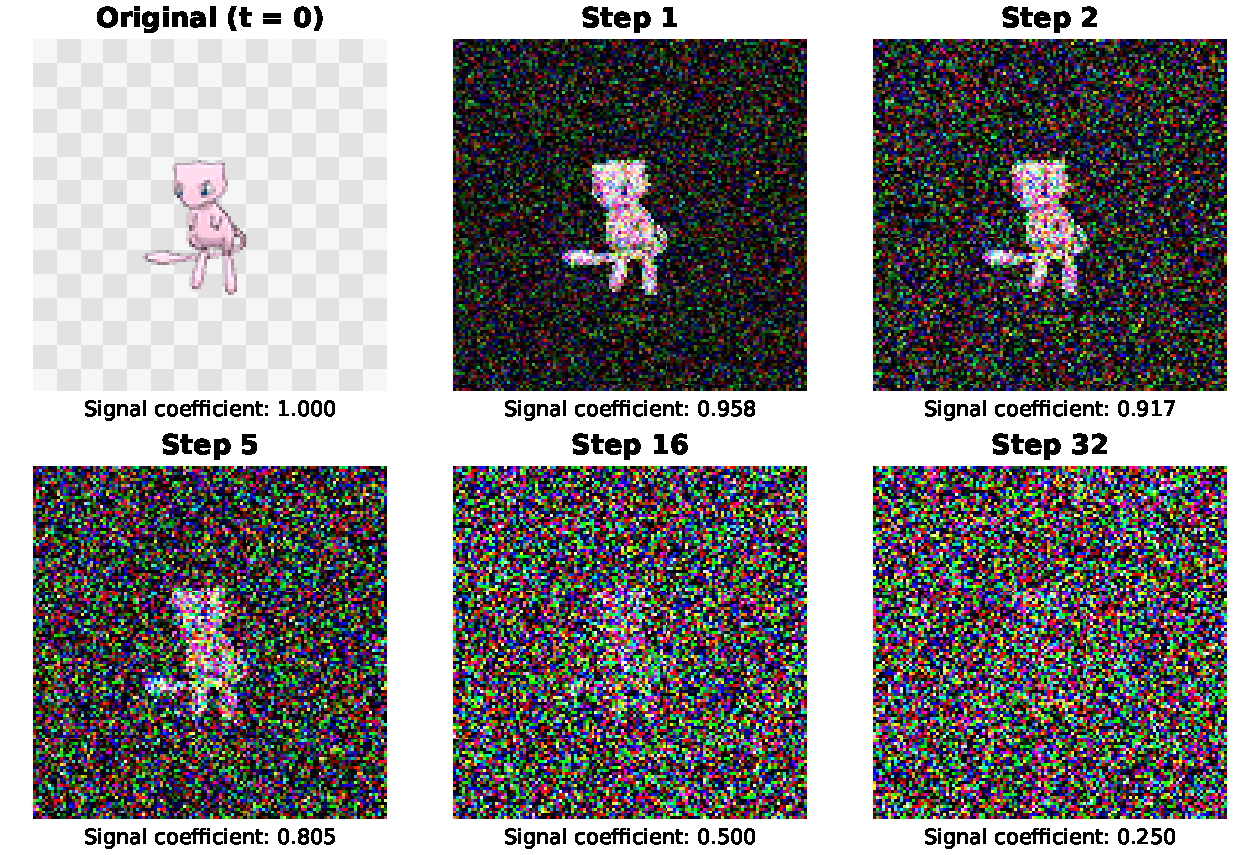
\includegraphics[width=0.95\linewidth]{generated/mew-stochastic-process.pdf}
\caption{Mew at steps $0,1,2,5,16,$ and $32$ along one reproducible stochastic
trajectory, with $\beta\approx0.082996$. Labels show the remaining signal
coefficient, not a percentage of recoverable information. The original is shown
with transparency on a checkerboard; later panels show opaque RGB previews
clipped only for display. All four RGBA channels evolve in the underlying
unclipped floating-point state. Mew is a training-set image chosen to explain the
process; this figure is separate from the held-out reconstruction examples.}
\label{fig:mew-process}
\end{figure}

Every earlier noise contribution is also scaled by the steps that follow it.
Their weighted sum is the accumulated noise $n_T$. Independent Gaussian
contributions combine into another Gaussian, giving a direct description of
the endpoint distribution.

\begin{proposition}[Gaussian endpoint]
In exact real arithmetic,
\begin{equation}
 x_T\mid x_0\sim\mathcal N(a_Tx_0,(1-a_T^2)I),\qquad
 x_T=a_Tx_0+n_T.
\end{equation}
\end{proposition}
\begin{proof}
Unrolling the recurrence gives
$n_T=\sum_{j=1}^{T}\sqrt\beta(1-\beta)^{(T-j)/2}\varepsilon_j$.
Independent Gaussian increments yield zero mean and covariance
$\beta\sum_{j=0}^{T-1}(1-\beta)^jI=[1-(1-\beta)^T]I$.
\end{proof}

Thus the 32-step teacher is $y=0.25x+n$, with
$n\sim\mathcal N(0,0.9375I)$. We sample this endpoint directly, avoiding the cost
of simulating all 32 increments. This matches the endpoint distribution, not an
individual unsaved noise trajectory. Given its realized $n$, the teacher has the
analytic inverse $x=(y-n)/0.25$. This known inverse provides a reference for
the learned maps. Our task is to approximate a specified transformation and
recover the same input; generative diffusion instead uses learned reverse
dynamics to sample plausible images \cite{ddpm,sde}.

\FloatBarrier
\subsection{Constructed inversion and numerical transport}
Our initial paper took a \emph{purely learned approach to forward and reverse
mapping}: two separately trained U-Net models learned the prescribed corruption
and reconstruction from paired examples \cite{original}. ``Purely learned''
describes those endpoint maps; the stochastic process providing their targets
was specified in advance. Reconstruction on the training collection showed
that the models could fit those examples, but left recovery of unseen images
unresolved. The reported evaluation did not establish either success or failure
on a held-out collection.

Making an image look noisy is easy; retaining a reliable way back to its exact
pixel values is the harder design requirement. Independently learning the two
directions does not guarantee that one undoes the other. An unconstrained forward
network can also discard distinctions between inputs that no decoder can restore.
We therefore introduce a structural constraint: each transformation block comes
with a known undo operation. Training determines how closely the resulting map
matches the stochastic target, while the architecture provides its inverse in
exact arithmetic.

The obstacle is easiest to see when a network computes an adjustment from the
original image and then changes every channel. To subtract that adjustment
later, we may need the original image---the very thing we are trying to recover.
Our channel split breaks this circular dependency: hold one group unchanged,
use it and the saved noise to calculate an adjustment to the other group, and
then switch roles. During reversal, the unchanged group is still available, so
we can calculate exactly the same adjustment again and subtract it.

For Mew, the first group contains red and green, and the second contains blue
and alpha. Both cover the entire image. The first block keeps red and green
available while changing blue and alpha; the next keeps the resulting blue and
alpha values available while changing red and green. Working backward restores
each group's earlier values when they are needed. Figure~\ref{fig:mew-coupling}
shows this sequence. The split is one convenient way to construct a reversible
learned map; the Gaussian teacher in Section~1.2 already has an analytic inverse
without a split. The coupling construction cannot repair information lost later
through clipping or coarse quantization, which we address below.

Formally, write the group held unchanged in a block as $u$ and the group being
updated as $v$. Each continuous coupling block applies
\begin{equation}
 u'=u,\qquad v'=sv+t_\theta(u,n),\qquad
 v=\frac{v'-t_\theta(u',n)}{s},\quad s\ne0.
 \label{eq:coupling}
\end{equation}
Alternating which half is updated and composing such blocks gives an explicit
inverse by reversing their order, following the coupling principle used in
Real NVP \cite{realnvp}. This algebraic property holds before training. Learning
controls target-map fidelity, not the existence of the inverse.

Because $u'=u$, the decoder can run the same conditioner network on $(u',n)$
to reproduce the forward adjustment, subtract it, and divide by $s$. The
conditioner itself need not be inverted. In our model, $s=0.5$ and four blocks
alternate the groups' roles, so both groups are changed twice. Decoding reverses
the block order, restoring the values needed for each preceding operation.
These four network blocks approximate the endpoint of the 32 stochastic steps
in Section~1.2; the two counts refer to different operations.

\begin{figure}[!htbp]
\centering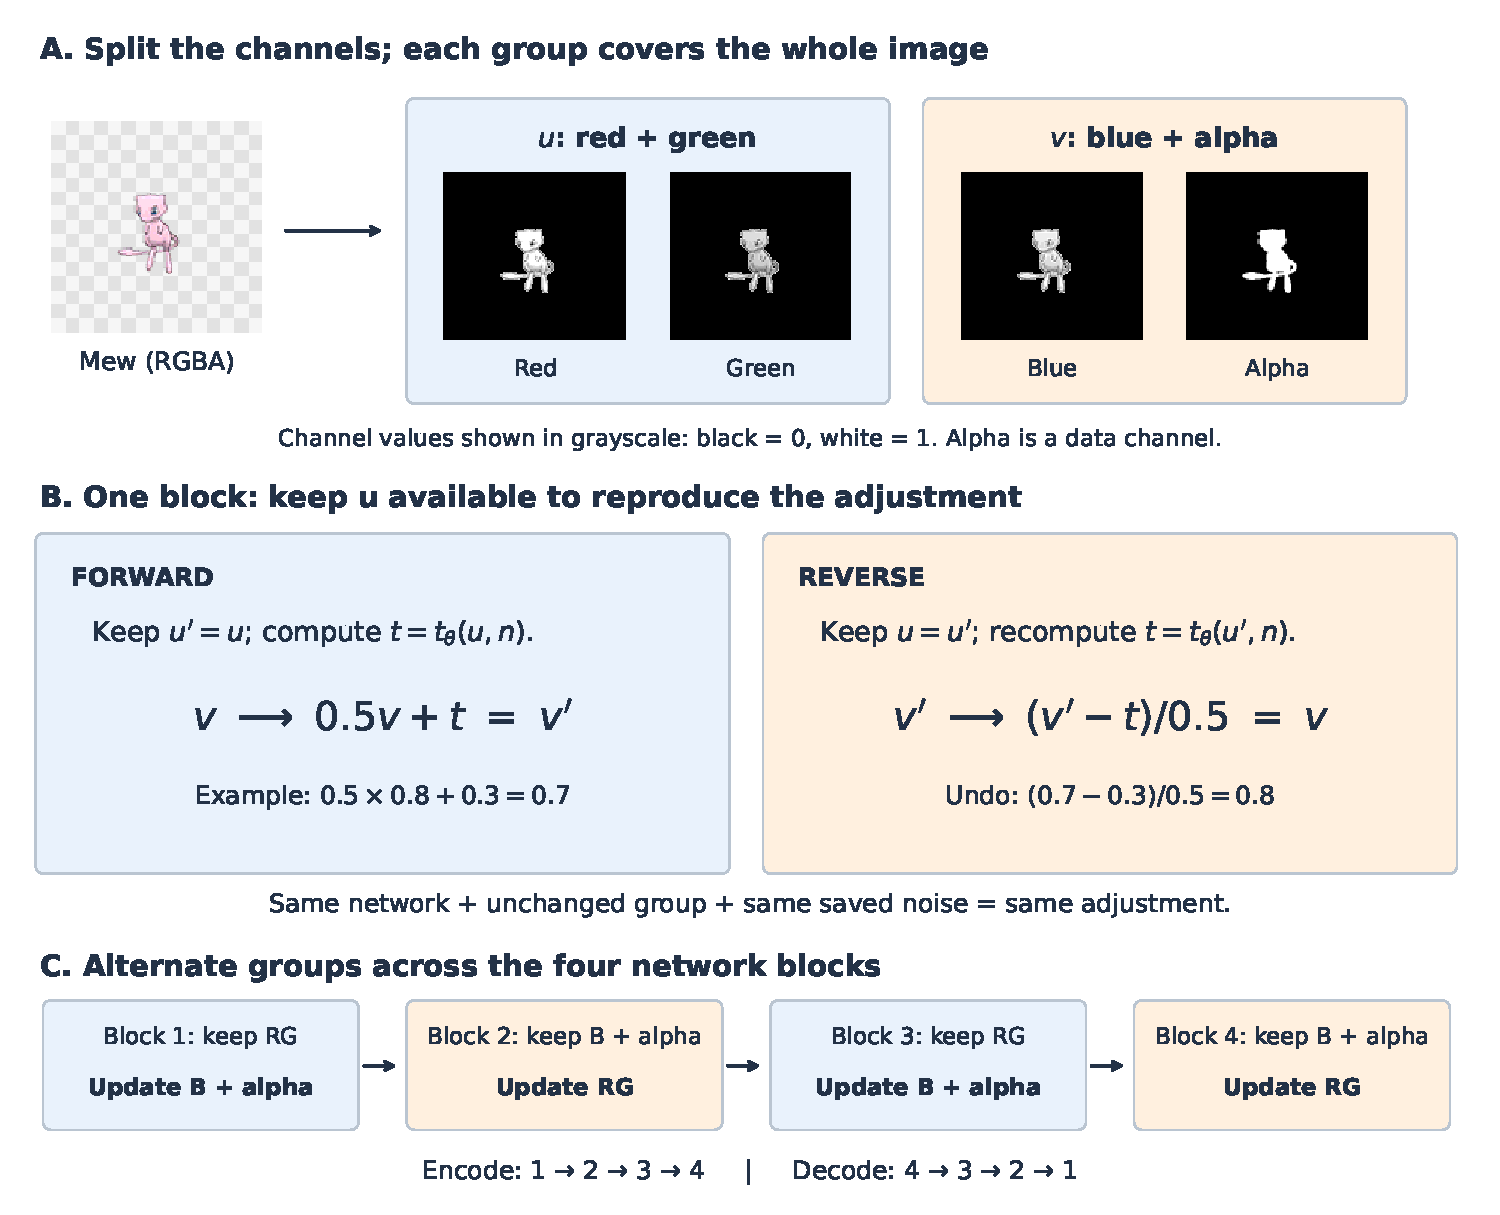
\includegraphics[width=0.95\linewidth]{generated/mew-coupling-diagram.pdf}
\caption{Constructed inversion using Mew's channel groups. (A) Original channel
values are displayed in grayscale, including alpha; both groups cover every
pixel. (B) One block holds $u$ unchanged while adjusting $v$. The decoder uses
the same conditioner and noise to reproduce the adjustment. The scalar example
shows how subtraction and division undo the update.
(C) Alternating the groups changes all four channels; reversing the block order
undoes the composition, up to floating-point error. A group is held unchanged
only within its current block.}
\label{fig:mew-coupling}
\end{figure}

An explicit inverse is useful only if storage retains the values it needs.
The original pipeline clipped its noisy RGB endpoint to $[0,1]$ and rounded it
to 8-bit PNG values \cite{original}; distinct floating-point values could therefore
become the same stored value. We instead serialize the Gaussian payload as
float32 NumPy arrays without clipping and decode from those arrays and the saved
conditioning field. This avoids the earlier destructive conversion, although
float32 still has finite precision. PNGs displayed as encrypted images are
clipped RGB previews only, not decodable substitutes for the stored RGBA payload.
For example, clipping sends both $1.2$ and $1.8$ to $1.0$. Once only $1.0$ is
stored, the decoder cannot tell which value preceded it, even with a perfectly
invertible network. Further training cannot restore that discarded distinction.

Finite arithmetic introduces reconstruction error. Normalizing byte values
divides them by 255, so adjacent levels are $1/255$ apart. For original byte-valued
inputs, error below half that spacing ($1/510$), allowing for input
rounding, suffices to recover the byte grid by nearest rounding. We measure this
directly rather than assuming it. The teacher inverse amplifies endpoint errors
by $1/a_T=4$; for example, a teacher-output error of $0.01$ becomes a recovered
input error of $0.04$. Small errors can nevertheless leave the rounded byte
unchanged: a recovered value of $127.99999$ in byte units rounds back to $128$.
The learned composition also depends on its conditioner sensitivities.
Exact-arithmetic invertibility therefore does not imply universal bitwise
portability across devices or library versions.

These changes address distinct limitations: the schedule controls attenuation,
coupling supplies an inverse, and the payload format preserves the numerical
values needed to use it. Their combined recovery results cannot be attributed
to channel splitting alone. Evaluation on images excluded from fitting, described
in Section~3, separately examines target approximation and round-trip recovery
beyond the training collection.

\FloatBarrier
\subsection{Geometry and algebra of reversible maps}
\label{sec:geometry}
Imagine nearby data points drawn on a coordinate grid. A reversible map can
bend the grid and change distances while keeping every point distinguishable.
Figure~\ref{fig:coupling-geometry} illustrates this with two coordinates:
\begin{equation*}
 C(u,v)=(u,\,0.5v+0.3u^2),\qquad
 C^{-1}(u',v')=(u',\,2(v'-0.3u'^2)).
\end{equation*}
The map compresses the vertical direction and shifts each vertical line by an
amount determined by its horizontal coordinate. The inverse straightens the
grid. For an image, the coordinates represent channel values across the whole
tensor; this picture illustrates a deformation of data space.
\begin{figure}[!htbp]
\centering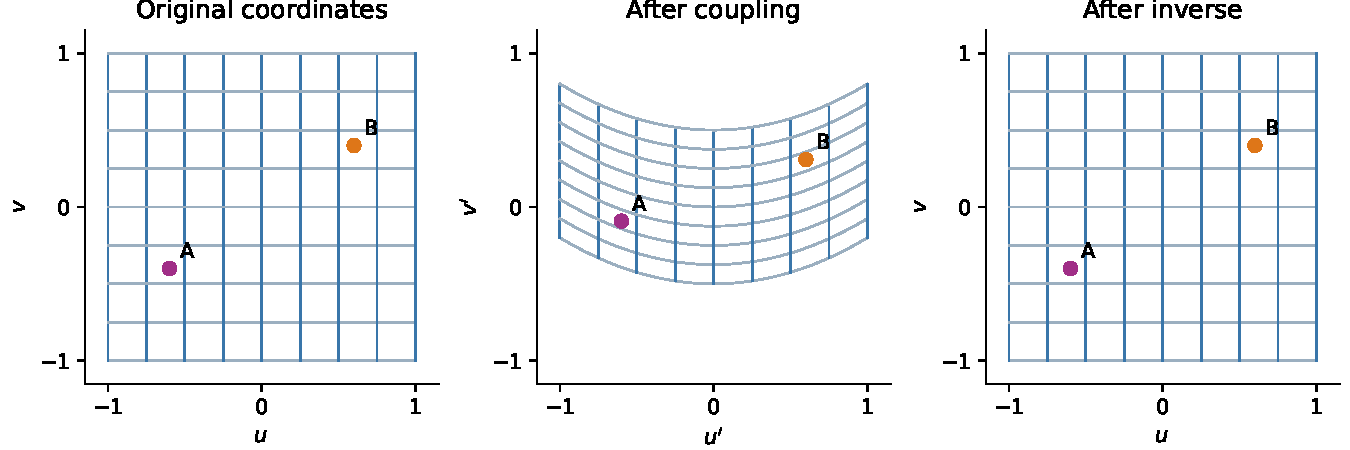
\includegraphics[width=\linewidth]{generated/coupling-geometry.pdf}
\caption{A two-coordinate coupling map and its inverse. The same two points,
A and B, are tracked through all three panels. Horizontal grid lines become
curves, vertical separation is halved, and every point remains recoverable.
Both directions are polynomial maps in this example.}
\label{fig:coupling-geometry}
\end{figure}

\paragraph{Differential geometry: smooth changes of coordinates.}
Fix the noise field $n$. The implemented conditioners combine affine
convolutions with the smooth activation $\operatorname{SiLU}(z)=z/(1+e^{-z})$.
Their coupling maps therefore have smooth forward and inverse operations on
$V$ in exact real arithmetic. Such a map is called a \emph{diffeomorphism}.
The coupling construction makes this property explicit \cite{realnvp}.
Zoom in on a tiny patch of the grid in Figure~\ref{fig:coupling-geometry}:
the Jacobian describes its local stretching and shearing. The magnitude of its
determinant gives the local area scale, or volume scale in higher dimensions.
For a block updating $q=N/2$ coordinates, its Jacobian is
\begin{equation}
 J_C(u,v)=
 \begin{pmatrix}
 I_q & 0\\
 \partial_u t_\theta(u,n) & sI_q
 \end{pmatrix},\qquad \det J_C=s^q\ne0.
 \label{eq:coupling-jacobian}
\end{equation}
In the two-coordinate example, the determinant is $0.5$: area is halved while
distinct points remain distinguishable. A nonzero determinant shows that no
local direction is collapsed. Global invertibility
follows from the explicit inverse in Equation~\ref{eq:coupling}; the determinant
alone would establish only local invertibility.

With four blocks and $s=0.5$, the full encoder satisfies
$|\det J_{\sigma_{\theta,n}}|=0.5^{4q}=0.25^N$, where
$\sigma_{\theta,n}(x)=\sigma_\theta(x,n)$. Thus the model contracts local volume while
preserving an inverse. The determinant's magnitude gives the product of local stretching
factors; individual directions can still be sensitive to perturbations. This
explains why numerical error requires measurement even when a smooth inverse
exists.

\paragraph{Composition and the algebraic viewpoint.}
Composition means applying one map after another. The notation is read from
right to left: $C_2\circ C_1$ applies $C_1$ first, then $C_2$. Undoing that
sequence requires undoing $C_2$ first, then $C_1$.
Writing the four blocks as $C_1,\ldots,C_4$, with fixed $n$, gives
\begin{equation}
 \sigma_{\theta,n}=C_4\circ C_3\circ C_2\circ C_1,\qquad
 \tau_{\theta,n}=C_1^{-1}\circ C_2^{-1}\circ C_3^{-1}\circ C_4^{-1},
\end{equation}
and $\tau_{\theta,n}\circ \sigma_{\theta,n}=\sigma_{\theta,n}\circ \tau_{\theta,n}
=\operatorname{id}_V$ in exact arithmetic, where the identity map
$\operatorname{id}_V$ leaves every input unchanged.
An endomorphism maps a space into itself while respecting the structure under
discussion; an automorphism additionally has an inverse respecting that same
structure. Here the structure is smoothness: in the category of smooth manifolds,
the encoder is an automorphism of the ambient tensor space $V$. This gives the
original endomorphism viewpoint a specific setting. The bounded
set of source images is only a subset of that space.

Algebraic geometry provides a related setting when the coordinate maps are
polynomials \cite{vandenessen}. If the conditioner $t_\theta(u,n)$ is polynomial
in $u$ for fixed $n$, then the coupling and its explicit inverse are polynomial,
so the block is a polynomial automorphism of real affine space. The two-coordinate
example above has this form, as does the fixed-noise Gaussian teacher
$x\mapsto0.25x+n$. The implemented SiLU conditioners supply smooth maps rather
than a polynomial parameterization. Polynomial conditioners offer an algebraic
variant for future experiments.

These distinctions also guide modality changes. Full continuous tensor spaces
related by a diffeomorphism must have the same real dimension. A larger carrier
space can instead contain an embedded copy of the source, with recovery defined
on that copy. For finite byte encodings, the corresponding requirement is enough
distinct stored carrier states for all admitted inputs. In each setting, the
geometric or algebraic inverse addresses recovery; Section~2 supplies the
separate secrecy argument for a keyed composition.

\section{Connection to the pursuit of post-quantum encryption}
\subsection{What quantum resistance would require}
Recovery and confidentiality answer different questions. Recovery asks whether
the intended receiver can get the original data back. Confidentiality asks
whether someone without the required secret can learn about it. In this
prototype, a second person given the model, payload, and saved noise can run
exactly the same decoder as the intended receiver. Accurate recovery therefore
does not establish a distinction between authorized and unauthorized access.

A useful way to think about confidentiality is a guessing experiment. An
observer knows two possible messages of equal length and receives a protected
version of one, chosen with equal probability. Without a revealing observation,
the observer can only guess with success probability $1/2$; indistinguishability
asks whether seeing the protected version improves that guess. Perfect secrecy
allows no improvement, while computational security requires any advantage
available within the specified resource limits to be negligible as the security
parameter grows.

The long-term objective is a system with efficient authorized inversion and
computationally difficult unauthorized recovery. Quantum resistance concerns
the capabilities of the adversary, not the absence of an inverse. Shor's
algorithms address factoring and discrete logarithms \cite{shor}; Grover's
algorithm supplies a quadratic speedup for unstructured search \cite{grover}.
Neither says that every invertible map is easily attacked, nor that visually
noisy or unfamiliar maps resist quantum computation. NIST's post-quantum
program evaluates explicit cryptographic constructions and security assumptions
against classical and quantum attacks \cite{nist}.

Our prototype is efficiently inverted by a classical computer given its public
weights and noise field. The reproducible random generator is not a cryptographic
key generator; its seed is experiment metadata. We release conditioning fields
to reproduce recovery and make no secrecy claim for them. Even a hidden Gaussian
field would not by itself establish perfect secrecy: the teacher's conditional
ciphertext distributions have input-dependent means. Residual structure and
distributional leakage require analysis beyond how noisy a rendered image looks.

\subsection{A future-system conjecture and a proof sketch}
The longer-term aim is to create that distinction through a specified secret-key
mechanism and to evaluate it against both classical and quantum adversaries.
Changing a message's outward form, as in the text-to-image example, adds a
possible concealment objective: an observer might not recognize the source
modality. Demonstrating that a carrier is indistinguishable from ordinary media
is a steganographic question, distinct from whether its hidden content is
cryptographically confidential. Neither property follows from representing the
data as a tensor or from changing its file format.
The following conjecture guides the search for a keyed construction. One route
is to combine an established secrecy mechanism with a learned carrier; the
sketch below gives a conditional result for this approach.
\begin{conjecture}[Research hypothesis; unproven]
Under suitable computational hardness assumptions, a future publicly specified
key-conditioned family of learned, information-preserving tensor transformations
can support efficient authorized recovery and confidentiality against
polynomial-time classical and quantum adversaries.
\end{conjecture}
To turn this conjecture into a computational security claim, a construction
must specify a security parameter,
secret-key distribution, public randomness or nonce rules, ciphertext format,
and an indistinguishability experiment with precisely defined oracle access.
At minimum, one should consider quantum computation with classical
chosen-plaintext queries; stronger quantum-query models require separate claims.
Models and architecture should be assumed public. Authentication, key exchange,
chosen-ciphertext resistance, and side-channel behavior are additional design
obligations, none supplied by reconstruction accuracy.

\paragraph{Sketch of Proof: preserving secrecy through a learned carrier.}
First protect the message, then change the form that carries it. If the protected
bits reveal no information about the message, expressing those same bits as an
image or waveform cannot create information about the message. The receiver
reverses the carrier transformation and then removes the protection using a
secret key.

Fix a public message length $L$ and a lossless representation
$M\in\{0,1\}^L$. The sender and receiver share a uniformly random secret pad
$K\in\{0,1\}^L$, independent of the message and the adversary's prior information.
Every transmission uses a fresh pad. For this keyed construction, let
$\sigma_\theta$ be a public, efficiently
computable learned map from $L$-bit strings to serialized image or audio
carriers. Its parameters are fixed independently of the secret message and pad.
Assume an efficient inverse $\tau_\theta$ satisfying
$\tau_\theta(\sigma_\theta(c))=c$ for every $c\in\{0,1\}^L$, including the effects of
serialization. The transmitted carrier is
\begin{equation}
 C=M\oplus K,\qquad Y=\sigma_\theta(C),\qquad
 M=\tau_\theta(Y)\oplus K,
 \label{eq:pad-carrier}
\end{equation}
where $\oplus$ is bitwise exclusive OR. The final identity establishes correctness.
The carrier can have any modality with sufficient capacity for these ciphertexts.

For example, a four-bit message $1010$ and pad $0110$ give
$1010\oplus0110=1100$. After reversing the carrier map, applying the same pad
recovers the message: $1100\oplus0110=1010$. XOR flips a message bit wherever
the pad has a $1$; applying those same flips twice restores the original bits.

For any fixed message, each possible ciphertext corresponds to exactly one
pad, and all pads are equally likely. The one-time-pad secrecy argument
\cite{shannon} therefore gives, for every $m,c$,
\begin{equation}
 \Pr[C=c\mid M=m]=\Pr[K=m\oplus c]=2^{-L}.
\end{equation}
Thus every message of length $L$ induces the same distribution of $C$. Applying
the fixed carrier map preserves that equality:
\begin{equation}
 \Pr[Y=y\mid M=m]
 =\sum_{c:\,\sigma_\theta(c)=y}2^{-L},
 \label{eq:carrier-secrecy}
\end{equation}
which is independent of $m$. An observer may know and reverse $\sigma_\theta$, but
this yields only the uniformly masked ciphertext $C$.

The equality also covers quantum computation on the observed classical carrier.
We write its distribution as a diagonal density operator,
\begin{equation}
 \rho_m=\sum_y\Pr[Y=y\mid M=m]\,|y\rangle\langle y|,
\end{equation}
where $|y\rangle\langle y|$ is the outer product of the basis vector
$|y\rangle$ representing output $y$ with its conjugate transpose $\langle y|$.
This outer product marks the diagonal position corresponding to output $y$:
it has a $1$ in that position and zeros elsewhere. Weighting each outer product
by its probability therefore places the output probabilities along the diagonal
of $\rho_m$. Since those probabilities are the same for every message,
we have $\rho_m=\rho_{m'}$ for every pair of messages. Identical input states
produce identical outcome distributions under every quantum computation and
measurement. The carrier therefore adds no distinguishing advantage, even with
unlimited computation. This argument concerns observation of classical
transmissions with independent pads; it assumes no access to the secret pad
or a decryption oracle. Public metadata must be fixed or generated from the
ciphertext and independent public randomness, so that the whole transmitted
record satisfies the same independence condition. Message length is public.

This construction establishes a conditional secrecy-preserving route toward
the conjecture. The pad supplies perfect secrecy, and the learned map supplies
the carrier representation. Its cost is an independently shared secret pad as
long as each message. Replacing the pad with a short pseudorandom seed would
require a separate computational security argument. Authentication and resemblance
to ordinary images or audio also require separate mechanisms or evidence.
The Gaussian noise used in our experiments is not a one-time pad, and measured
round-trip accuracy does not establish the assumed exact carrier inverse for
every possible bit string. Constructing such a carrier, or bounding its decoding
error, is the next implementation step.

\section{Architecture, training, and Pok\'emon experiments}
\subsection{Model and training protocol}
Replacing the original pair of independently trained U-Nets \cite{original},
the network has four alternating channel-coupling blocks with shared forward
and inverse parameters. Each conditioner uses
a $3\times3$ convolution from six channels (two unchanged image channels plus
four noise channels) to 32 channels, SiLU, a second $3\times3$ 32-channel
convolution, SiLU, and a $1\times1$ output convolution to two channels.
There are 44,296 trainable parameters. Each half is updated twice; the fixed
scale $s=0.5$ makes its total multiplicative attenuation $0.25$. This builds the
teacher's known overall scaling into the architecture: training learns the
additive adjustments needed to match its endpoint. Supplying this part of the
target structure in advance is the model's known-scale inductive bias.

The original models classified each RGB value into one of 256 byte bins
\cite{original}. Because our transport retains continuous-valued RGBA tensors,
we use regression against the floating-point targets. The loss is the sum of
forward and reverse mean squared errors:
\begin{equation}
 \mathcal L=\mathbb E\left[\|\sigma_\theta(x,n)-T_\omega(x)\|^2_{\mathrm{mean}}
 +\|\tau_\theta(T_\omega(x),n)-x\|^2_{\mathrm{mean}}\right].
\end{equation}
Three independent runs use seeds 17, 29, and 43, each with 2,000 optimizer updates,
effective batch size 16, and microbatch size four. AdamW uses learning rate
$3\times10^{-4}$, weight decay $10^{-5}$, and gradient clipping at one.
These are optimizer updates, not 2,000 passes through the dataset. All coupling
arithmetic uses FP32 with TF32 disabled and deterministic cuDNN settings.

The original study fitted and evaluated the same paired collection
\cite{original}. To distinguish fitting that collection from performance on
images excluded from training, we use separate training, validation, and test
sets. Training fits parameters, validation selects checkpoints, and test
evaluation measures the selected models. The 809 native $120\times120$ sprites
come from the \emph{Pokemon sprite images} dataset shared by Kaggle user
yehongjiang \cite{pokemon-data} and retain their RGBA channels. The inherited
split contains 647 training, 81 validation, and 81 test images, grouping decoded
duplicates, name variants, and available evolution links. The supplied evolution
metadata are incomplete. Training samples sprites with replacement and fresh
noise. Validation every 100 updates ranks checkpoints first by the excess of
round-trip MAE over $10^{-6}$, treating errors at or below that tolerance as tied,
and then by summed forward/reverse target MAE. All three
checkpoints are frozen and hashed before this campaign's test evaluation.
The same test set was previously examined during exploratory work; consequently
this is a follow-up evaluation, not a previously untouched confirmatory holdout.
Further tuning would require fresh confirmatory data.

Uniform static was not included in training because the earlier fixed-budget
comparison did not improve with it. That finding does not rule out structured
synthetic data or exposure-matched augmentation. Independent test streams of 32
static images and nine structured probes supplement the 81 Pok\'emon test images.

\subsection{Losses, target fidelity, and reconstruction}
An accurate round trip can coexist with an imperfect match to the teacher.
Consider a scalar example with $x=0.8$ and saved noise $n=0.1$. The teacher gives
$T(x,n)=0.25x+n=0.30$. Suppose a learned map instead gives
$\sigma(x,n)=0.25x+n+0.01=0.31$, with constructed inverse
$\tau(z,n)=(z-n-0.01)/0.25$. Then
\begin{equation*}
\begin{aligned}
 \text{forward error:}&& |0.31-0.30|&=0.01,\\
 \text{reverse error:}&& |\tau(0.30,0.1)-0.8|=|0.76-0.8|&=0.04,\\
 \text{round-trip error:}&& |\tau(0.31,0.1)-0.8|&=0.
\end{aligned}
\end{equation*}
The map perfectly reverses its own output even though it differs from the
teacher's transformation.

Forward error measures agreement with the prescribed teacher; reverse error
decodes teacher outputs. Round-trip error instead decodes the network's own
serialized output. Reporting these errors separately shows both target fidelity
and recovery. MAE is normalized to original pixel units
on $[0,1]$, including all RGBA entries. Foreground RGB errors use the original
nonzero-alpha mask and are included in the accompanying results.

Our saved untrained controls make the same distinction experimentally.
Table~\ref{tab:training-control} compares the randomly initialized networks
with their selected trained checkpoints on the same validation collection.
Every image was already recovered exactly after rounding before training,
although the target errors were large. Training substantially reduced those
target errors. The round-trip property comes from the architecture; training
teaches its additive functions to match the prescribed process.
\begin{table}[!htbp]
\centering\small\begin{tabular}{lrrr}
\toprule
Model state & Forward MAE & Reverse MAE & \shortstack{Exact RGBA\\images (\%)} \\
\midrule
Before training & 0.77634 & 3.11343 & 100.0 \\
After training & 0.00924 & 0.03691 & 100.0 \\
\bottomrule
\end{tabular}

\caption{Before and after training on the 81 validation Pok\'emon images.
Entries are means across seeds 17, 29, and 43. ``After'' uses each seed's
validation-selected checkpoint. ``Exact RGBA images'' is the percentage of whole
images with every channel byte recovered after rounding; all three seeds attain 100\%
both before and after training.}
\label{tab:training-control}
\end{table}

\begin{figure}[ht]
\centering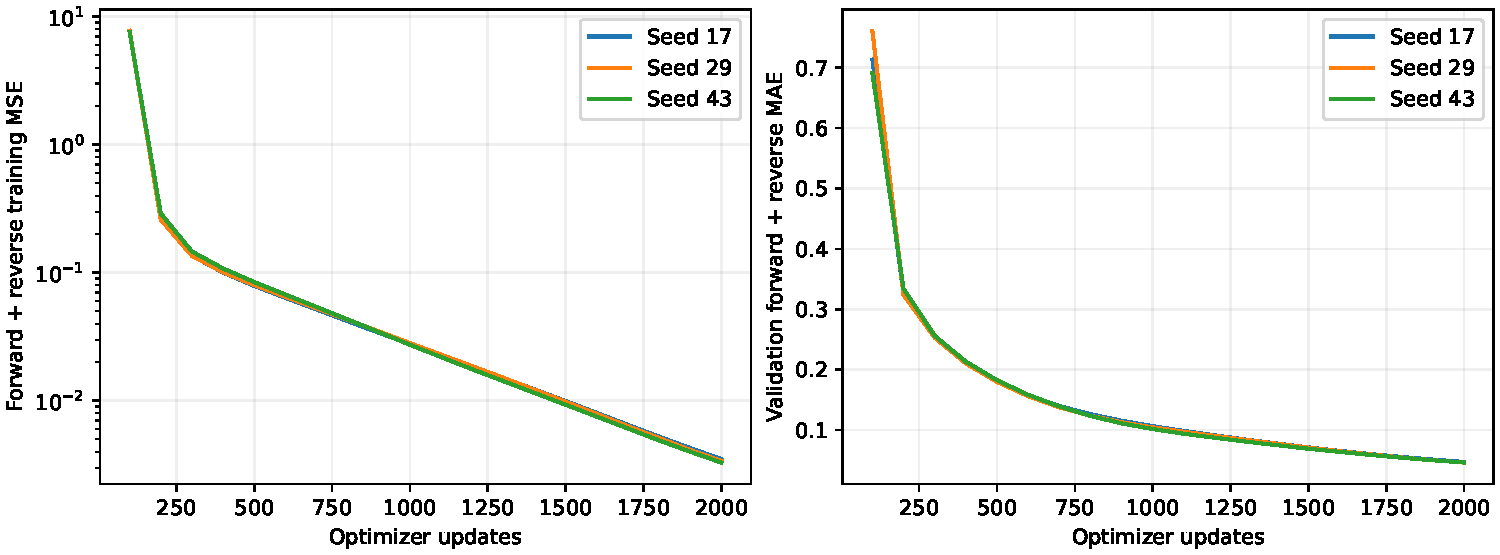
\includegraphics[width=\linewidth]{generated/learning-curves.pdf}
\caption{Training loss averaged over successive 100-update intervals, and
validation target error. Each curve follows one training seed.}
\end{figure}

\begin{table}[!htbp]
\centering\small\setlength{\tabcolsep}{4pt}\begin{tabular}{rrrrrr}
\toprule
Seed & Best update & Forward MAE & Reverse MAE & Round-trip MAE & \shortstack{Exact RGBA\\images (\%)} \\
\midrule
17 & 2000 & 0.00934 & 0.03736 & $1.5\times10^{-7}$ & 100.0 \\
29 & 2000 & 0.00918 & 0.03666 & $1.43\times10^{-7}$ & 100.0 \\
43 & 2000 & 0.00922 & 0.03679 & $1.45\times10^{-7}$ & 100.0 \\
\bottomrule
\end{tabular}

\caption{Results on the 81 test Pok\'emon images, shown separately for each
training seed. MAEs use normalized RGBA values. ``Exact RGBA images'' is the
percentage of entire images recovered byte-for-byte after rounding.}
\label{tab:test-results}
\end{table}
\FloatBarrier
Mean foreground-only RGB reverse-target MAE at 32 steps was 0.04199. The minimum exact RGBA image-recovery rate across all three seeds and all three test domains was \ExactRate\%. The largest floating-point round-trip error across those runs was $\WorstError$. These measurements describe the evaluated images and runtime; they are not a universal finite-precision guarantee.

Per-image and per-domain results, untrained validation controls, selected update
numbers, environment records, source code, and frozen checkpoints are available
in the reproducibility repository \cite{reproduction}. Seed variation describes
training variation and is not a population confidence interval.

\FloatBarrier
\subsection{Comparison with the 16-step study}
Moving to 32 steps produced a tradeoff: measured RGB correlation with the input
was lower and forward-target agreement improved, while reverse-target agreement
worsened. Exact byte recovery of the models' own outputs remained 100\% in the
tested domains. The stronger attenuation therefore trades lower measured
correlation for greater difficulty decoding the teacher's outputs.

The 16-step exploratory study followed the original paper and already used
coupling and float transport. It used the same model capacity, training split,
update budget, and seeds as the present experiment, with endpoint signal
coefficient $0.5$. The 32-step model is newly
trained with coefficient $0.25$. The following table reports mean and sample
standard deviation across three seeds on the same test images. The comparison
changes the teacher, so the metrics describe two task difficulties rather than a
competition against an identical target.

\begin{table}[!htbp]
\centering\small\begin{tabular}{rrrrr}
\toprule
Steps & Signal & Forward MAE & Reverse MAE & Round-trip MAE \\
\midrule
16 & 0.5 & $0.0164\pm0.00012$ & $0.0328\pm0.00024$ & $7.58\times10^{-8}\pm1\times10^{-9}$ \\
32 & 0.25 & $0.00924\pm8.6\times10^{-5}$ & $0.0369\pm0.00037$ & $1.46\times10^{-7}\pm3.5\times10^{-9}$ \\
\bottomrule
\end{tabular}

\caption{Target and round-trip MAEs on the same 81 test Pok\'emon images.
Entries are mean $\pm$ sample standard deviation across three training seeds.
Signal is the teacher's coefficient on the original input. The two schedules
define different targets.}
\label{tab:step-comparison}
\end{table}

The mean forward-plus-reverse target MAE decreased from \OldTargetMAE{} at 16 steps to \NewTargetMAE{} at 32 steps. Separately, forward-target MAE changed from 0.01641 to 0.00924, while reverse-target MAE changed from 0.03283 to 0.03694. The two directions should therefore also be assessed separately.


\begin{figure}[ht]
\centering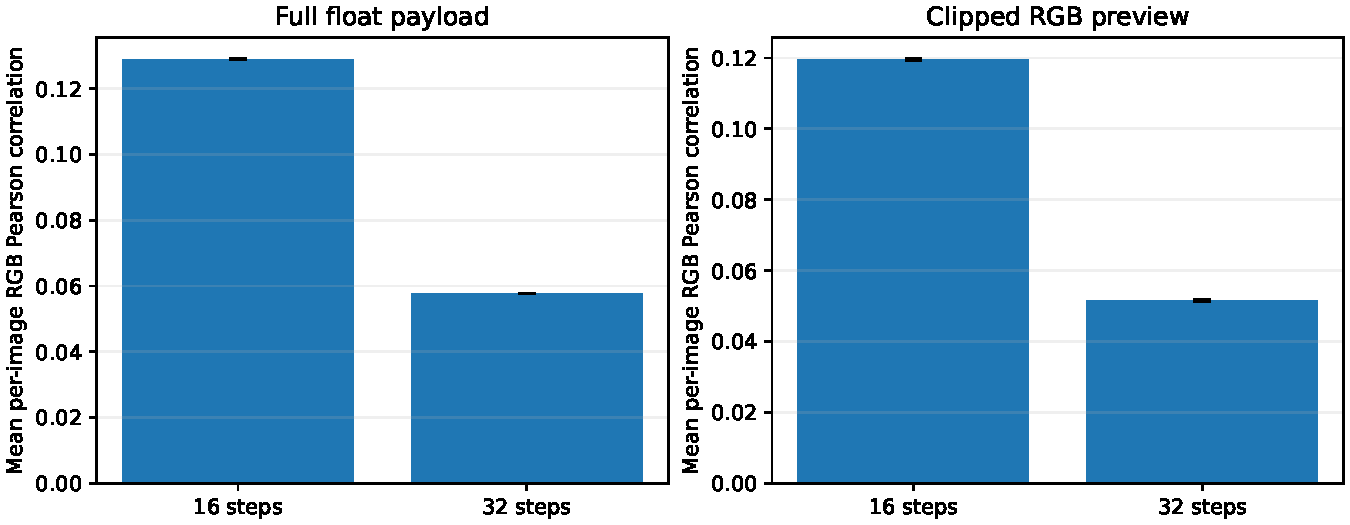
\includegraphics[width=0.75\linewidth]{generated/visibility.pdf}
\caption{Post-hoc descriptive correlation between original RGB and each learned
output, using full float payloads and clipped previews. Error bars show seed
standard deviation. Lower correlation does not establish confidentiality or
rule out nonlinear identification or reconstruction attacks.}
\end{figure}
Mean preview correlation is \OldCorrelation{} for 16 steps and \NewCorrelation{}
for 32 steps. Noise fields use matching underlying standard-normal streams for
the comparison. Residual recognizable structure remains a question for
identification and reconstruction tests beyond this correlation summary.

\FloatBarrier
\subsection{Actual image examples and resource costs}
Figure~\ref{fig:examples} illustrates one predetermined test image; the appendix
contains the first 25 in manifest order, without selection for appearance or
reconstruction quality. Checkerboards display original and reconstructed
transparency. The encrypted preview shows opaque clipped RGB; the saved float
payload also contains transformed alpha.
\begin{figure}[!htbp]
\centering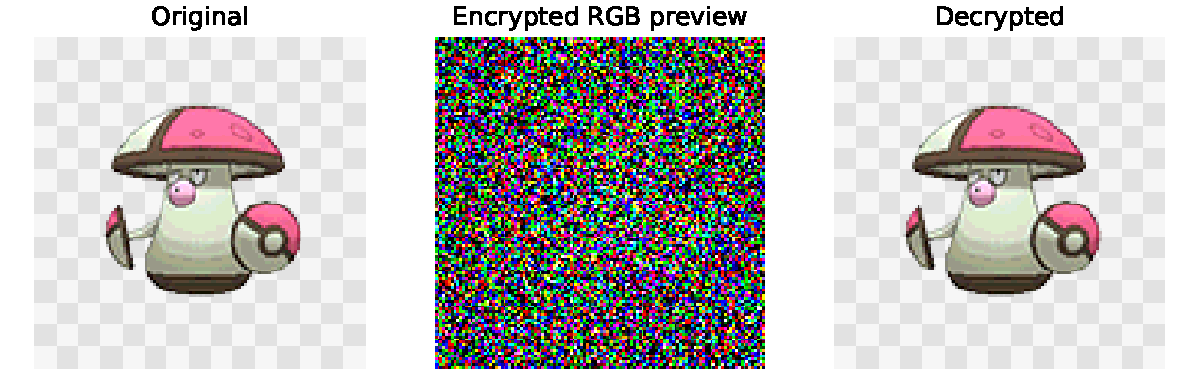
\includegraphics[width=0.70\linewidth]{generated/example-single.pdf}
\caption[First held-out test image]{\protectAmoonguss, the first test image in manifest order (seed 17). Float round-trip MAE is $1.51\times10^{-7}$; all RGBA bytes are recovered exactly after rounding.

The center panel is a clipped preview; recovery uses the full float payload
and saved noise.}
\label{fig:examples}
\end{figure}

On the RTX 5070 with 12 GB VRAM, training took
\MinMinutes--\MaxMinutes{} minutes per run, excluding validation and checkpoint
overhead. Peak PyTorch tensor allocation was approximately \MaxVRAM{} MiB per run; driver
memory and other processes are excluded. Timing describes this shared workstation.
The float32 RGBA payload and noise field each occupy 230,400 raw bytes, excluding
container overhead and shared model weights. Replacing the noise field with a
seed would require generator and stream-position metadata and separate security
analysis.

The central finding is that target approximation and reliable recovery can be
designed and evaluated separately: training improves agreement with the
stochastic teacher, while coupling and float transport preserve the way back
to the source pixels. The measured gains address the original pipeline's
recovery limitations; they establish neither an advantage over the analytic
inverse nor cross-device bitwise compatibility.
The text-to-image and image-to-audio paths in Figure~\ref{fig:cross-modal} are
concrete next experiments: their first recovery criterion would be exact source
bytes after serialization of the carrier. Carrier realism and resilience to
format conversions would need additional tests, alongside a specified keyed
construction and independent attacker evaluations for security claims.

\clearpage
\appendix
\section{All 25 predetermined test examples}
Every panel below uses the seed-17 model and the saved float payload. Encrypted
panels are display-only RGB previews. All 25 examples were chosen by manifest
order before examining this campaign's outputs.
\begin{figure}[ht!]\centering
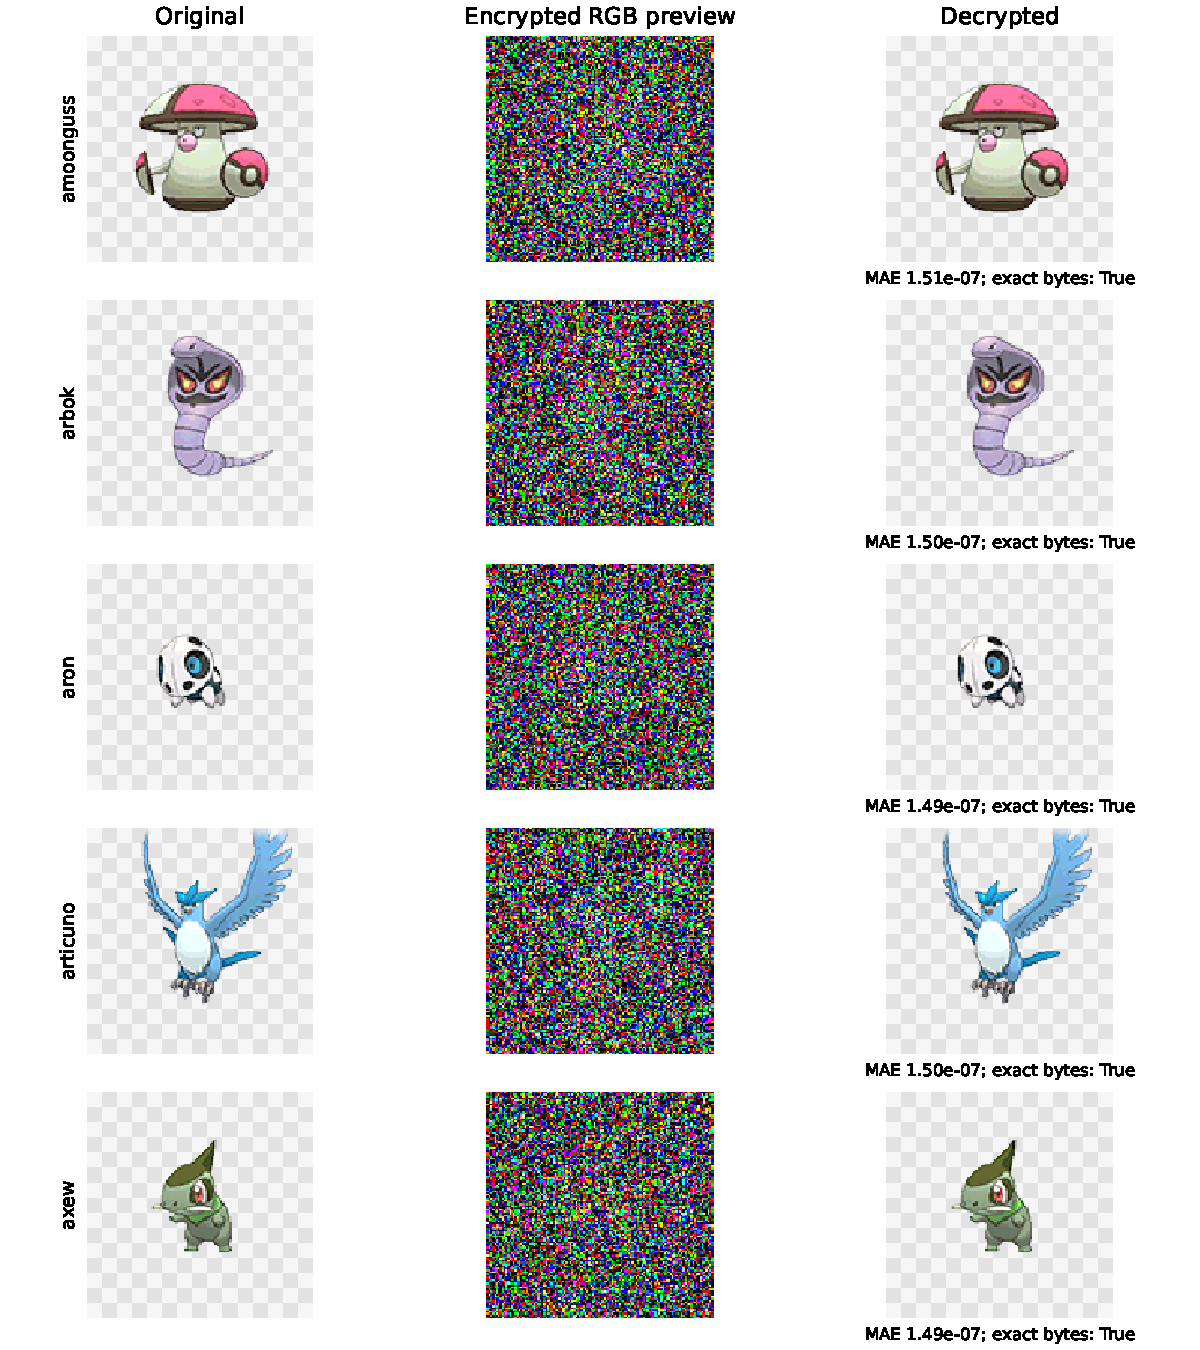
\includegraphics[width=0.85\linewidth]{generated/examples-01.pdf}
\caption{Test examples 1--5.}\end{figure}
\clearpage
\begin{figure}[p]\centering
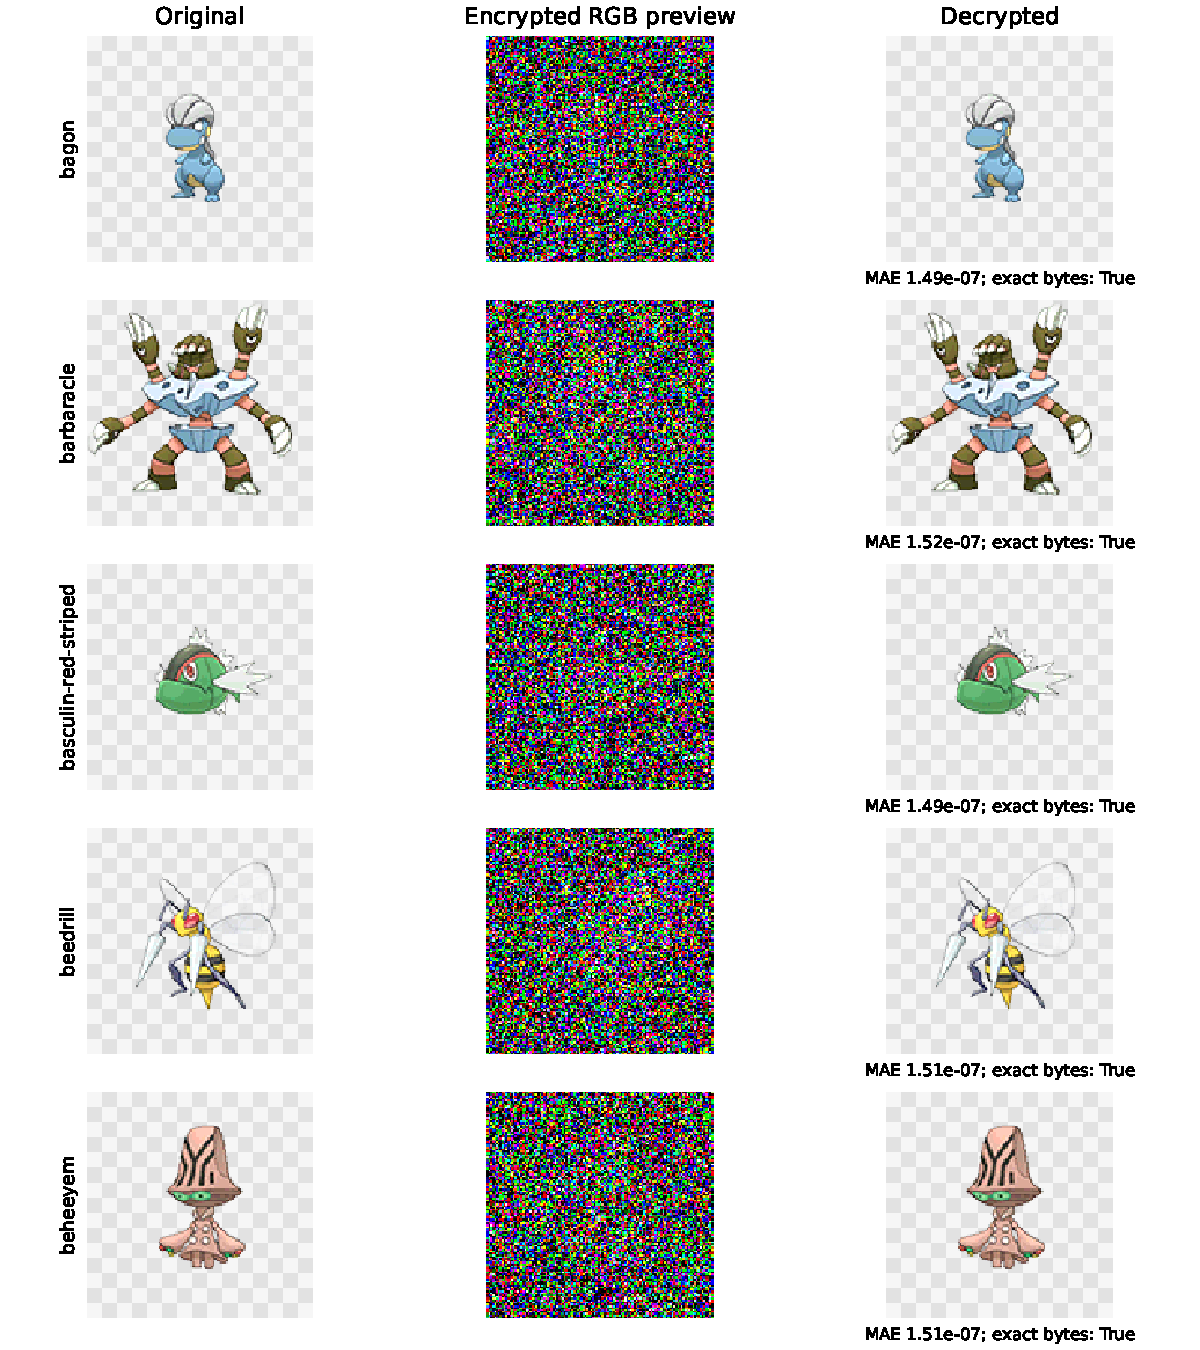
\includegraphics[width=0.85\linewidth]{generated/examples-02.pdf}
\caption{Test examples 6--10.}\end{figure}
\clearpage
\begin{figure}[p]\centering
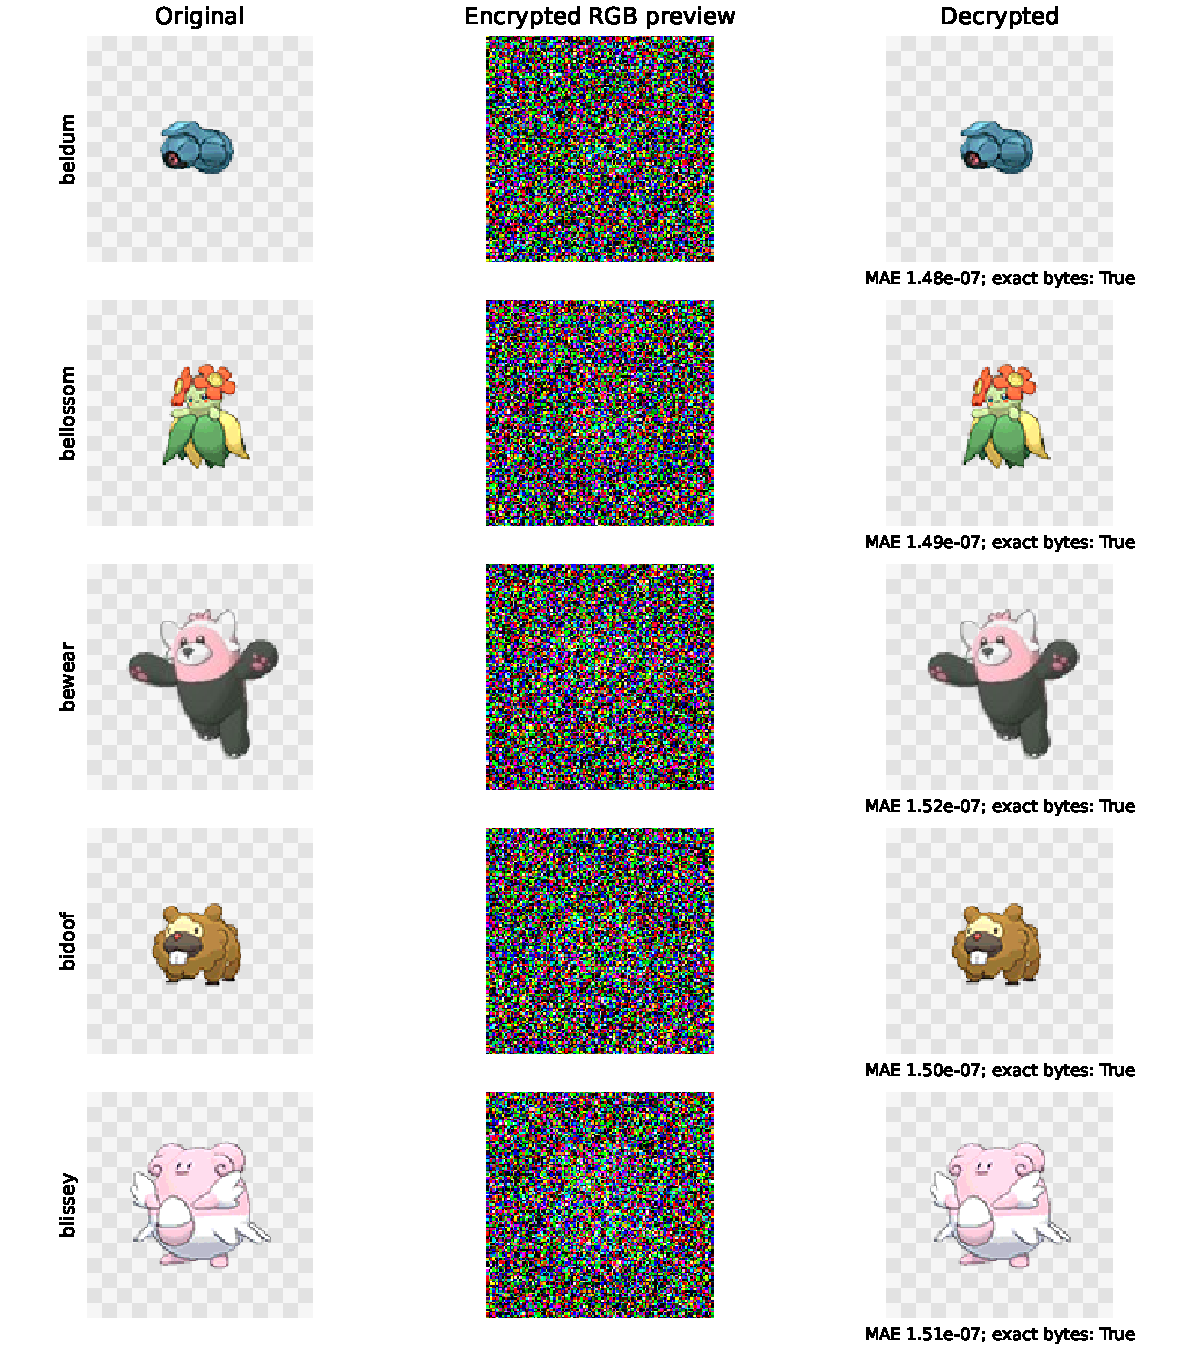
\includegraphics[width=0.85\linewidth]{generated/examples-03.pdf}
\caption{Test examples 11--15.}\end{figure}
\clearpage
\begin{figure}[p]\centering
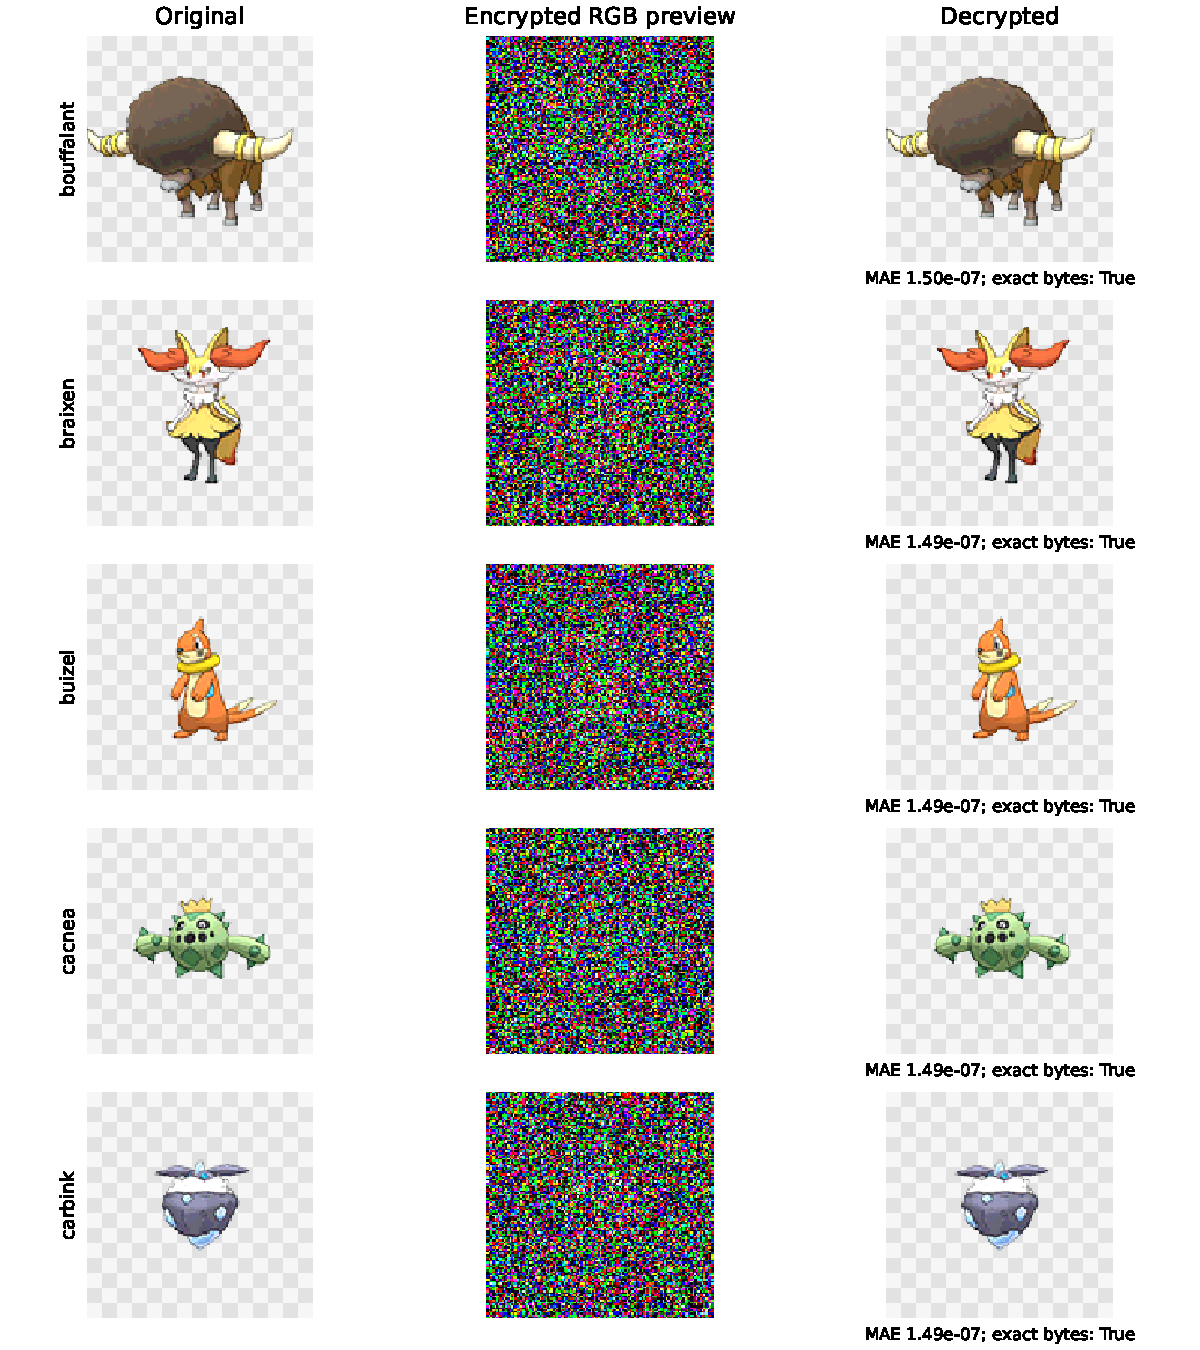
\includegraphics[width=0.85\linewidth]{generated/examples-04.pdf}
\caption{Test examples 16--20.}\end{figure}
\clearpage
\begin{figure}[p]\centering
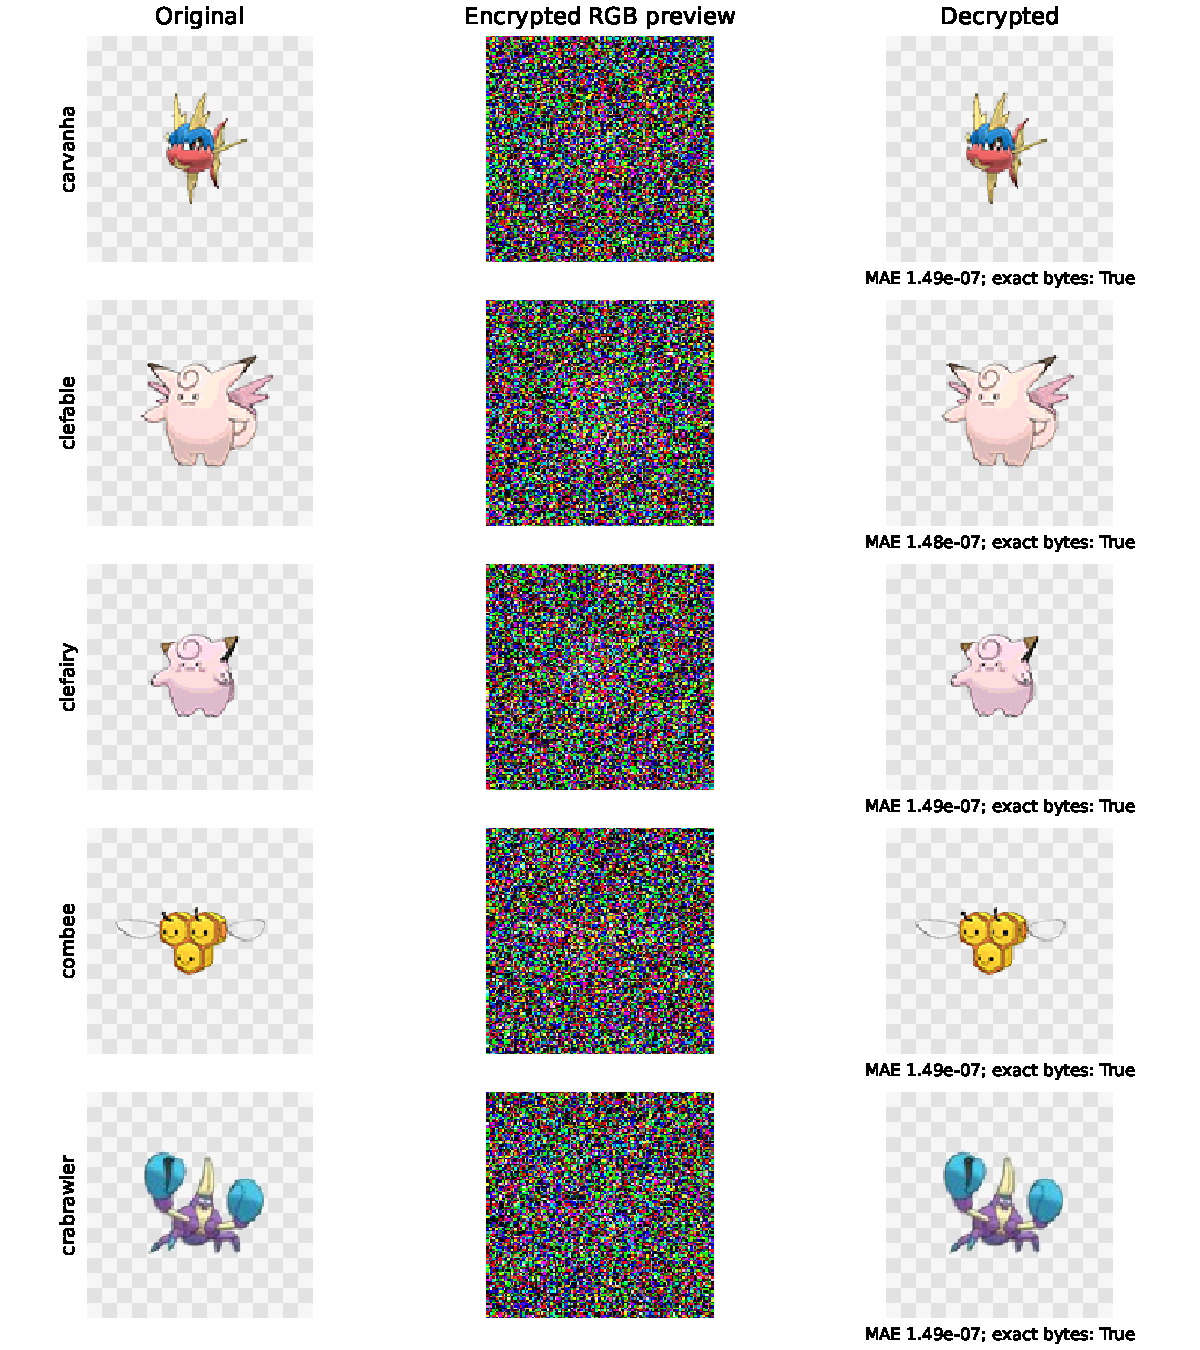
\includegraphics[width=0.85\linewidth]{generated/examples-05.pdf}
\caption{Test examples 21--25.}\end{figure}
\clearpage
\begin{thebibliography}{99}
\bibitem{original} S. Cavazos. Learned Encrypter-Decrypter Models for
Diffusion-Like Image Encryption: A Machine-Learning Approach Based on
Stochastic Processes. Alshival.AI, original manuscript and implementation.
\url{https://github.com/Alshival-Ai/alshicrypt-multimodal}.
\bibitem{realnvp} L. Dinh, J. Sohl-Dickstein, and S. Bengio.
Density estimation using Real NVP. ICLR, 2017.
\url{https://arxiv.org/abs/1605.08803}.
\bibitem{vandenessen} A. van den Essen. Polynomial Automorphisms and the
Jacobian Conjecture. S\'eminaires et Congr\`es, 2:55--81, 1997.
\url{https://smf.emath.fr/publications/polynomial-automorphisms-and-jacobian-conjecture}.
\bibitem{hidden} J. Zhu, R. Kaplan, J. Johnson, and L. Fei-Fei.
HiDDeN: Hiding Data with Deep Networks. ECCV, 2018.
\url{https://arxiv.org/abs/1807.09937}.
\bibitem{ddpm} J. Ho, A. Jain, and P. Abbeel.
Denoising Diffusion Probabilistic Models. NeurIPS, 2020.
\url{https://arxiv.org/abs/2006.11239}.
\bibitem{sde} Y. Song et al. Score-Based Generative Modeling through Stochastic
Differential Equations. ICLR, 2021.
\url{https://arxiv.org/abs/2011.13456}.
\bibitem{shor} P. W. Shor. Polynomial-Time Algorithms for Prime Factorization and
Discrete Logarithms on a Quantum Computer. SIAM Journal on Computing, 1997.
\url{https://arxiv.org/abs/quant-ph/9508027}.
\bibitem{grover} L. K. Grover. A fast quantum mechanical algorithm for database
search. STOC, 1996. \url{https://arxiv.org/abs/quant-ph/9605043}.
\bibitem{nist} NIST. Post-Quantum Cryptography: Frequently Asked Questions.
Accessed October 2026. \url{https://csrc.nist.gov/Projects/Post-Quantum-Cryptography/faqs}.
\bibitem{shannon} C. E. Shannon. Communication Theory of Secrecy Systems.
Bell System Technical Journal, 28(4):656--715, 1949.
\url{https://doi.org/10.1002/j.1538-7305.1949.tb00928.x}.
\bibitem{pokemon-data} yehongjiang. Pokemon sprite images. Kaggle dataset.
\url{https://www.kaggle.com/datasets/yehongjiang/pokemon-sprites-images}.
\bibitem{reproduction} S. Cavazos. Alshicrypt multimodal, October 2026:
source code, frozen checkpoints, and experimental records.
\url{https://github.com/Alshival-Ai/alshicrypt-multimodal-oct-2026}.
\end{thebibliography}
\end{document}
